\documentclass[french]{report}
 
\usepackage[utf8]{inputenc}
\usepackage[T1]{fontenc}
\usepackage{babel}
\usepackage{hyperref}
\usepackage[a4paper, margin=3cm]{geometry}
\usepackage{graphicx}
\usepackage{float}
\usepackage[bottom]{footmisc}
\usepackage{gensymb}
\usepackage[normalem]{ulem}

\setlength{\parindent}{0em}
\setlength{\parskip}{1em}

\begin{document}

\title{Serado Annonces}
\author{David Alvarez Restrepo <\href{mailto:devdav@pm.me}{devdav@pm.me}>}
\maketitle

\chapter{Analyse}

\section{Définition des besoins}
Deux acteurs utiliserons le système:
\begin{itemize}
    \item Directeur de Serado
    \item Possesseurs de l'application mobile \og Serado Annonce\fg{}
\end{itemize}

Le directeur de Serado pourra insérer des annonces, afin que ces dernières
soient consultable à partir de l'application mobile. Il pourra également insérer
d'autres informations (informations générales) avec des liens (par exemple. référence vers un article), qui
n'ont pas de rapport avec les annonces.

Les utilisateurs de l'application mobile pourront consulter les annonces ainsi que
consulter les informations générales. Les missions les plus proches apparaîtront
en premier dans la liste. Ils pourront aussi trier les annonces selon leur
ancienneté. Il n'y aura qu'une seule liste, les annonces temporaires et fixes étant
mélangées. Sur la liste qui affichera les annonces, il n'y aura peu d'informations.
Lorsque l'utilisateur clique sur une annonce, il aura une vue détaillée de cette
dernière.

L'application devra aussi contenir une partie qui référencera les sites suivants:
\begin{itemize}
    \item employee-de-maison.ch
    \item Pôle-Formation
    \item Hotellerie-Restauration
\end{itemize}
\vspace{1em}
Enfin, l'application devra être disponible sur iPhone et sur Android.

\section{Charte graphique}
À part le logo qui pourra être réutilisé pour les applications mobiles, il n'y a
aucune contraintes.

\section{Analyse du système}
Cette section décrit plus en détail et schématiquement ce qui a été dit dans la
section précédente.

Le diagramme de cas d'utilisations permet d'avoir un aperçu des acteurs et de leurs actions au sein du
système.

Il y a deux acteurs: le \textbf{directeur} et les \textbf{employés}. Le \textbf{directeur}
peut déjà \textbf{insérer/modifier/supprimer une annonce} à partir de
\textit{WordPress} (Ce qui est déjà existant avant l'analyse est entouré d'un
rectangle gris). En ce qui concerne le cas d'utilisation
\textbf{insérer/modifier/supprimer une info générale}, Le mieux sera de l'intégrer
à \textit{WordPress}. Si nous n'y parvenons pas, soit un autre système
sera créé, soit cette fonctionnalité sera mise de côté.

L'\textbf{employé} pourra consulter les \textbf{annonces} (ainsi que les détails de ces dernières)
et consulter les \textbf{informations générales} et leurs détails. 

\begin{figure}[H]
    \centering
    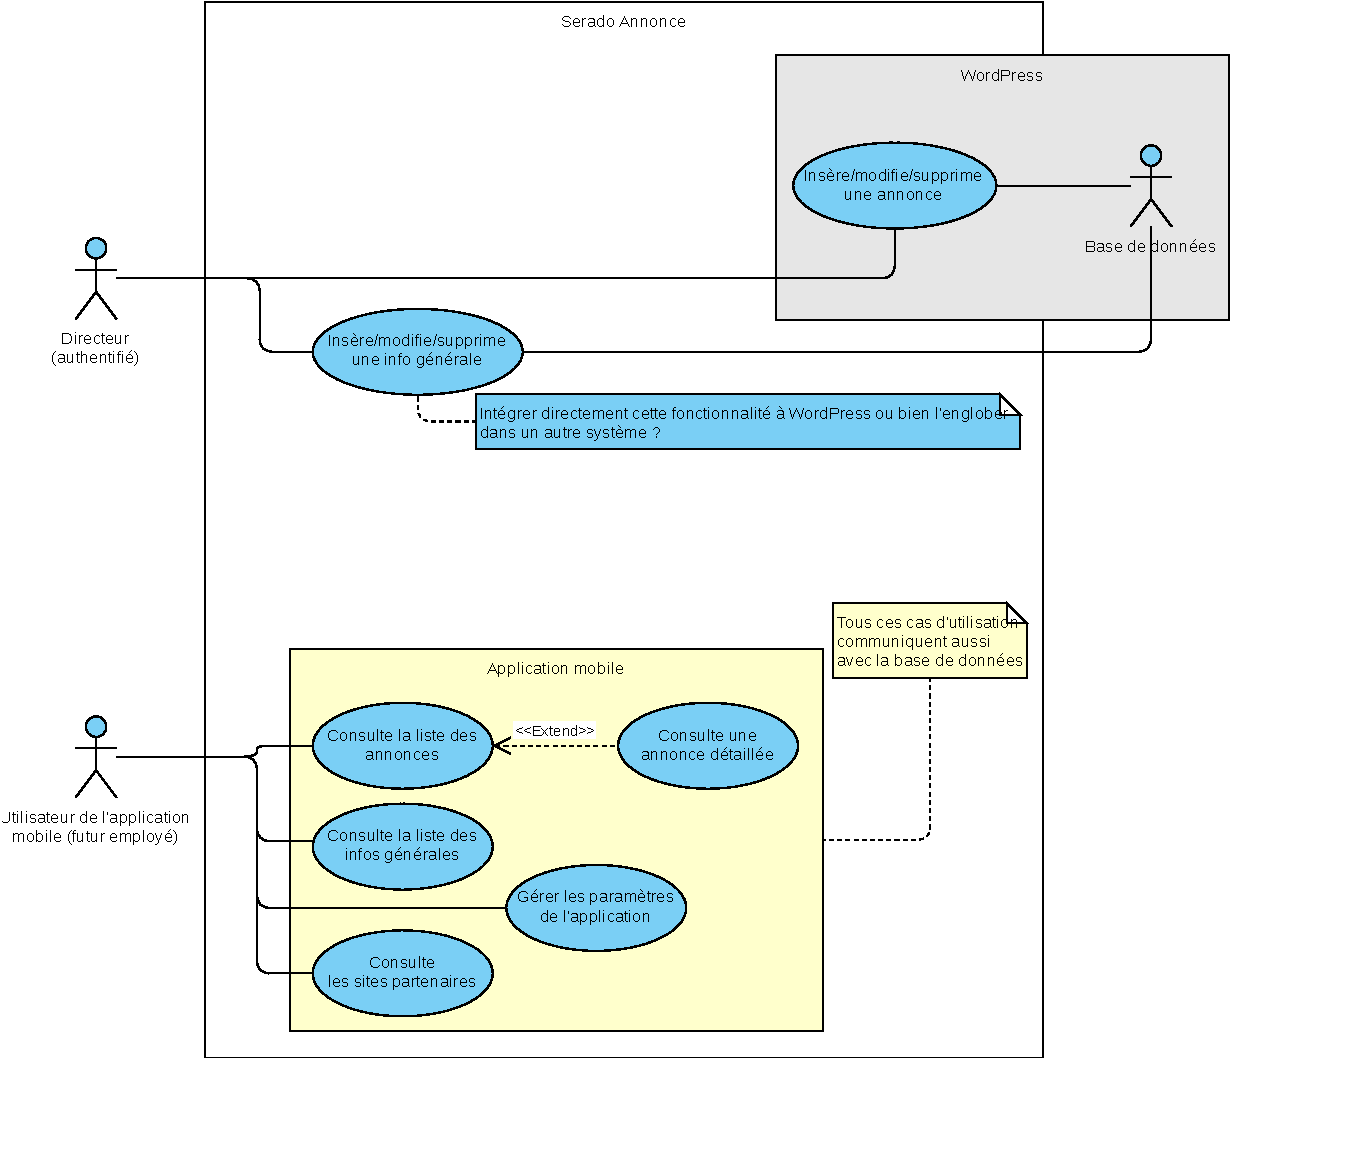
\includegraphics[width=\textwidth]{../diags/serado_uc.pdf}
    \caption{Diagramme de cas d'utilisation}
    \label{fig:use_case_diagram}
\end{figure}

\subsection{Analyse de l'existant}

Le cas d'utilisation \textbf{Insérer/modifier/supprimer} existe déjà et il est
effectué à partir de \textit{WordPress}. Vu qu'il existe, inutile de créer un autre
système qui effectuera la même chose. L'idéal est d'utiliser ce qui existe déjà. Il
va donc falloir trouver un moyen de récupérer ces informations afin de les afficher
dans l'application mobile.

\textbf{Remarque:} ces informations peuvent être visualisées à la page 
\url{https://serado.ch/offres-demploi/}

Il y a deux moyens pour récupérer ces informations:
\begin{enumerate}
    \item Étudier \textit{WordPress} afin de voir comment mettre en place une
    API\footnote{Application Programming Interface} qui servent les entités
    \textbf{offres d'emploi} au format JSON.
    \item Analyser le contenu de l'URL \url{https://serado.ch/offres-demploi/} afin
    de créer un objet JSON à partir du contenu de ce lien.
\end{enumerate}
\vspace{1em}

\sout{Puisque la personne qui gère \textit{WordPress} est absente cette semaine
(11.11.2019), nous partirons plutôt sur la méthode n\degree2.} C'est la méthode
n\degree1 qui a été finalement faite.

Ensuite, puisque on utilise \textit{WordPress} pour insérer les offres d'emploi,
l'idéal serait de aussi l'utiliser pour insérer les informations générales.
Autrement il faudrait créer un autre sytème entier uniquement pour cela, ce qui n'est
pas rentable. Cette fonctionnalité pourra être effectuée à partir de la deuxième semaine
(18.11.2019) du projet, lorsque la personne qui gère \textit{WordPress} sera disponible.

Pour résumer, il faudrait utiliser \textit{WordPress} pour le cas d'utilisation
\textbf{Insérer/modifier/supprimer une info générale} et voir s'il est possible de
créer une API qui renvoie uniquement les données demandées (et non pas toute la
page HTML).


\section{Choix des technologies}

\subsection{Langage de programmation / Framework}
Le but est de livrer une application mobile qui soit compatible avec \textit{iOS}
et \textit{Android}. On va donc utiliser un langage qui permet la programmation
d'application \textit{cross-platform}. J'en connais deux:
\begin{itemize}
    \item \textit{React Native}
    \item \textit{Ionic}
\end{itemize}
Je choisis \textbf{\textit{Ionic}} pour les raisons suivantes:
\begin{enumerate}
    \item Pas besoin d'avoir une application native (60 FPS\footnote{Frame Per Second}),
    une \textit{WebView} à 30 FPS est suffisant.
    \item \textit{Ionic} est basé sur \textit{Angular}, que je trouve plus \og
    propre \fg{} que \textit{React Native}.
    \item \textit{Ionic} offre aussi une application pour \textit{Windows Phone} (même si
    cela représente moins de 1\% du marché).
    \item Le projet \textit{Ionic} pourra être adapté très facilement afin de créer
    un site web mobile, et ainsi toucher même les personnes n'ayant pas l'application
    installée.
\end{enumerate}
\vspace{1em}

En ce qui concerne l'\textbf{interface administrateur}, nous continuerons d'utiliser
\textit{WordPress}.


\subsection{API tierces}

L'application devra avoir accès au services externes ci-dessous.

\subsubsection{Google Maps API}

Afin d'afficher une \textit{map} (carte), l'API de google sera utilisée:
\url{https://developers.google.com/maps/documentation/javascript/tutorial}. Afin de
pouvoir l'utiliser, il faudra rentrer un numéro de carte de crédit. L'utilisation
de l'API est gratuite: \url{https://cloud.google.com/maps-platform/pricing/sheet/}. 

ATTENTION: pendant la première année un crédit de 300\$/mois est offert pour
l'utilisation des services, ce qui devrait être suffisant pour l'entreprise, en
partant du principe qu'il n'y aura pas énormément d'utilisateur. Il me semble
qu'après cette année, certains services sont restreints, voir: 
\url{https://cloud.google.com/free/docs/gcp-free-tier}.

Deux API sont utilisées:
\begin{description}
    \item[Geocoding API] Trouve les coordonnées GPS d'un lieu à partir de son adresse.
    \item[Maps JavaScript API] Affiche la carte, ainsi que plusieurs marqueurs.  
\end{description}
\vspace{1em}

La \textbf{Geocoding API} est normalement peu utilisé, elle récupère les
coordonnées des annonces, puis les stocke dans la mémoire interne. Elle sera donc
appelée une fois par annonce par utilisateur. La \textbf{Maps JavaScript API} quant
à elle est beaucoup utilisée. Elle est appelée à chaque fois qu'un utilisateur
clique sur une annonce.

Si il s'avère que l'utilisation gratuite est dépassée à cause de cela, je propose
deux solutions:
\begin{enumerate}
    \item Payer pour l'API et regarder les frais sur un mois, et, continuer ainsi selon les frais.
    \item Utiliser \textbf{Maps Embed API} (son utilisation est normalement complètement gratuite). Voir \url{https://developers.google.com/maps/documentation/embed/guide}
\end{enumerate}
La dernière option permet seulement d'afficher une map avec un seul marqueur. On
perdrait alors la fonctionnalité qui permettait à l'utilisateur de voir à la fois
sa position et celle de l'annonce sur la carte.

Voir ce lien pour les autre soptimisations possibles: \url{https://developers.google.com/maps/optimization-guide}

\subsubsection{WP Job Manager}

Nous aurons aussi besoin de récupérer la liste des offres d'emplois. Pour cela, nous
utiliserons l'API du plugin \textit{WP Job Manager}:
\begin{description}
    \item[Liste des jobs] \url{https://www.serado.ch/wp-json/wp/v2/job-listings}
    \item[Détail d'un job] \url{https://www.serado.ch/wp-json/wp/v2/job-listings/{id}} 
\end{description}
\vspace{1em}

Les liens ci-dessus ont été trouvés à l'adresse suivante: \url{https://github.com/Automattic/WP-Job-Manager/pull/1628}

\subsection{Déploiement}

Le framework \textit{Ionic} permettra de créer les exécutables (\verb|.apk| et
\verb|.app|). Il faudra ensuite les mettre dans leur store respectif 
\textit{Play Store} et \textit{App Store} afin que les futurs utilisateurs puissent
la télécharger. Pour ce faire, voici la procédure:
\begin{description}
    \item[Play Store] Créer un compte \textit{Android Developer} (25\$, à vie), puis poster
    l'exécutable (\verb|.apk|) et attendre que \textit{Google} valide l'application.
    Procédure: \url{https://ionicframework.com/docs/publishing/play-store}.
    \item[App Store] Créer un compte \textit{Apple Developer Program} (100\$/année),
    puis suivre la procédure: \url{https://ionicframework.com/docs/publishing/app-store}.
\end{description}


\section{Permissions}
L'application demandera à l'utilisateur de le localiser afin de:
\begin{enumerate}
    \item Trier les annonces en fonction de la distance
    \item Afficher l'utilisateur sur une carte. La carte sera affichée dans chaque
    annonce détaillée. Ceci permettra de voir la distance entre l'utilisateur et le
    lieu de l'emploi en un clin d'\oe il
\end{enumerate}


\chapter{Conception}
Dans ce chapitre, les cas d'utilisation seront décrit plus en détail (fiches
descriptives). Il comprendra aussi les maquettes UI\footnote{User Interface}.

\section{Fiches descriptives}
Les fiches descriptives sont dans le dossier \verb|no_code/fd/|. Il y en a une par
cas d'utilisation. Elles sont au format \textit{Markdown} (à ouvrir directement dans
\textit{GitHub} ou bien dans le programme \textit{Typora }). Chaque fiche descriptive
a une référence vers un ou plusieurs écrans présents dans les maquettes.

\section{Navigation}
La navigation se fera à l'aide d'un \textit{drawer}. Ceci permet de ne pas surcharger
toutes les pages avec un \textit{bottom navigation} par exemple.

Les pages suivantes seront accessibles à partir du \textit{ďrawer}:
\begin{itemize}
    \item Liste des annonces
    \item Liste des information générales
    \item List des partenaires
\end{itemize}
\vspace{1em}

\textbf{L'application affichera l'écran "Liste des annonces" par défaut.}

\begin{figure}[H]
    \centering
    \begin{minipage}{.4\textwidth}
        \centering
        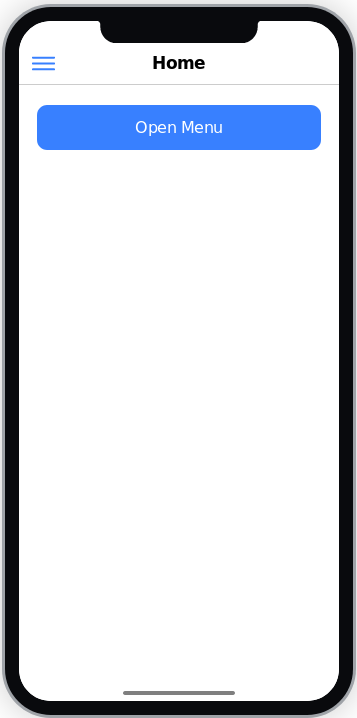
\includegraphics[width=0.7\linewidth]{../imgs/drawer-closed}
        \caption{Drawer fermé}
    \end{minipage}
    \begin{minipage}{0.4\textwidth}
        \centering
        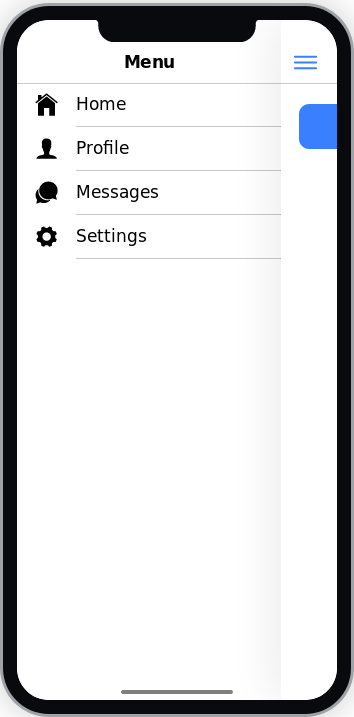
\includegraphics[width=0.7\linewidth]{../imgs/drawer-opened}
        \caption{Drawer ouvert}
    \end{minipage}
\end{figure}

\section{Maquettes}
Les maquettes sont des fichiers au format \verb|pdf| dans le dossier
\verb|no_code/mocks/|.

\begin{figure}[H]
    \centering
    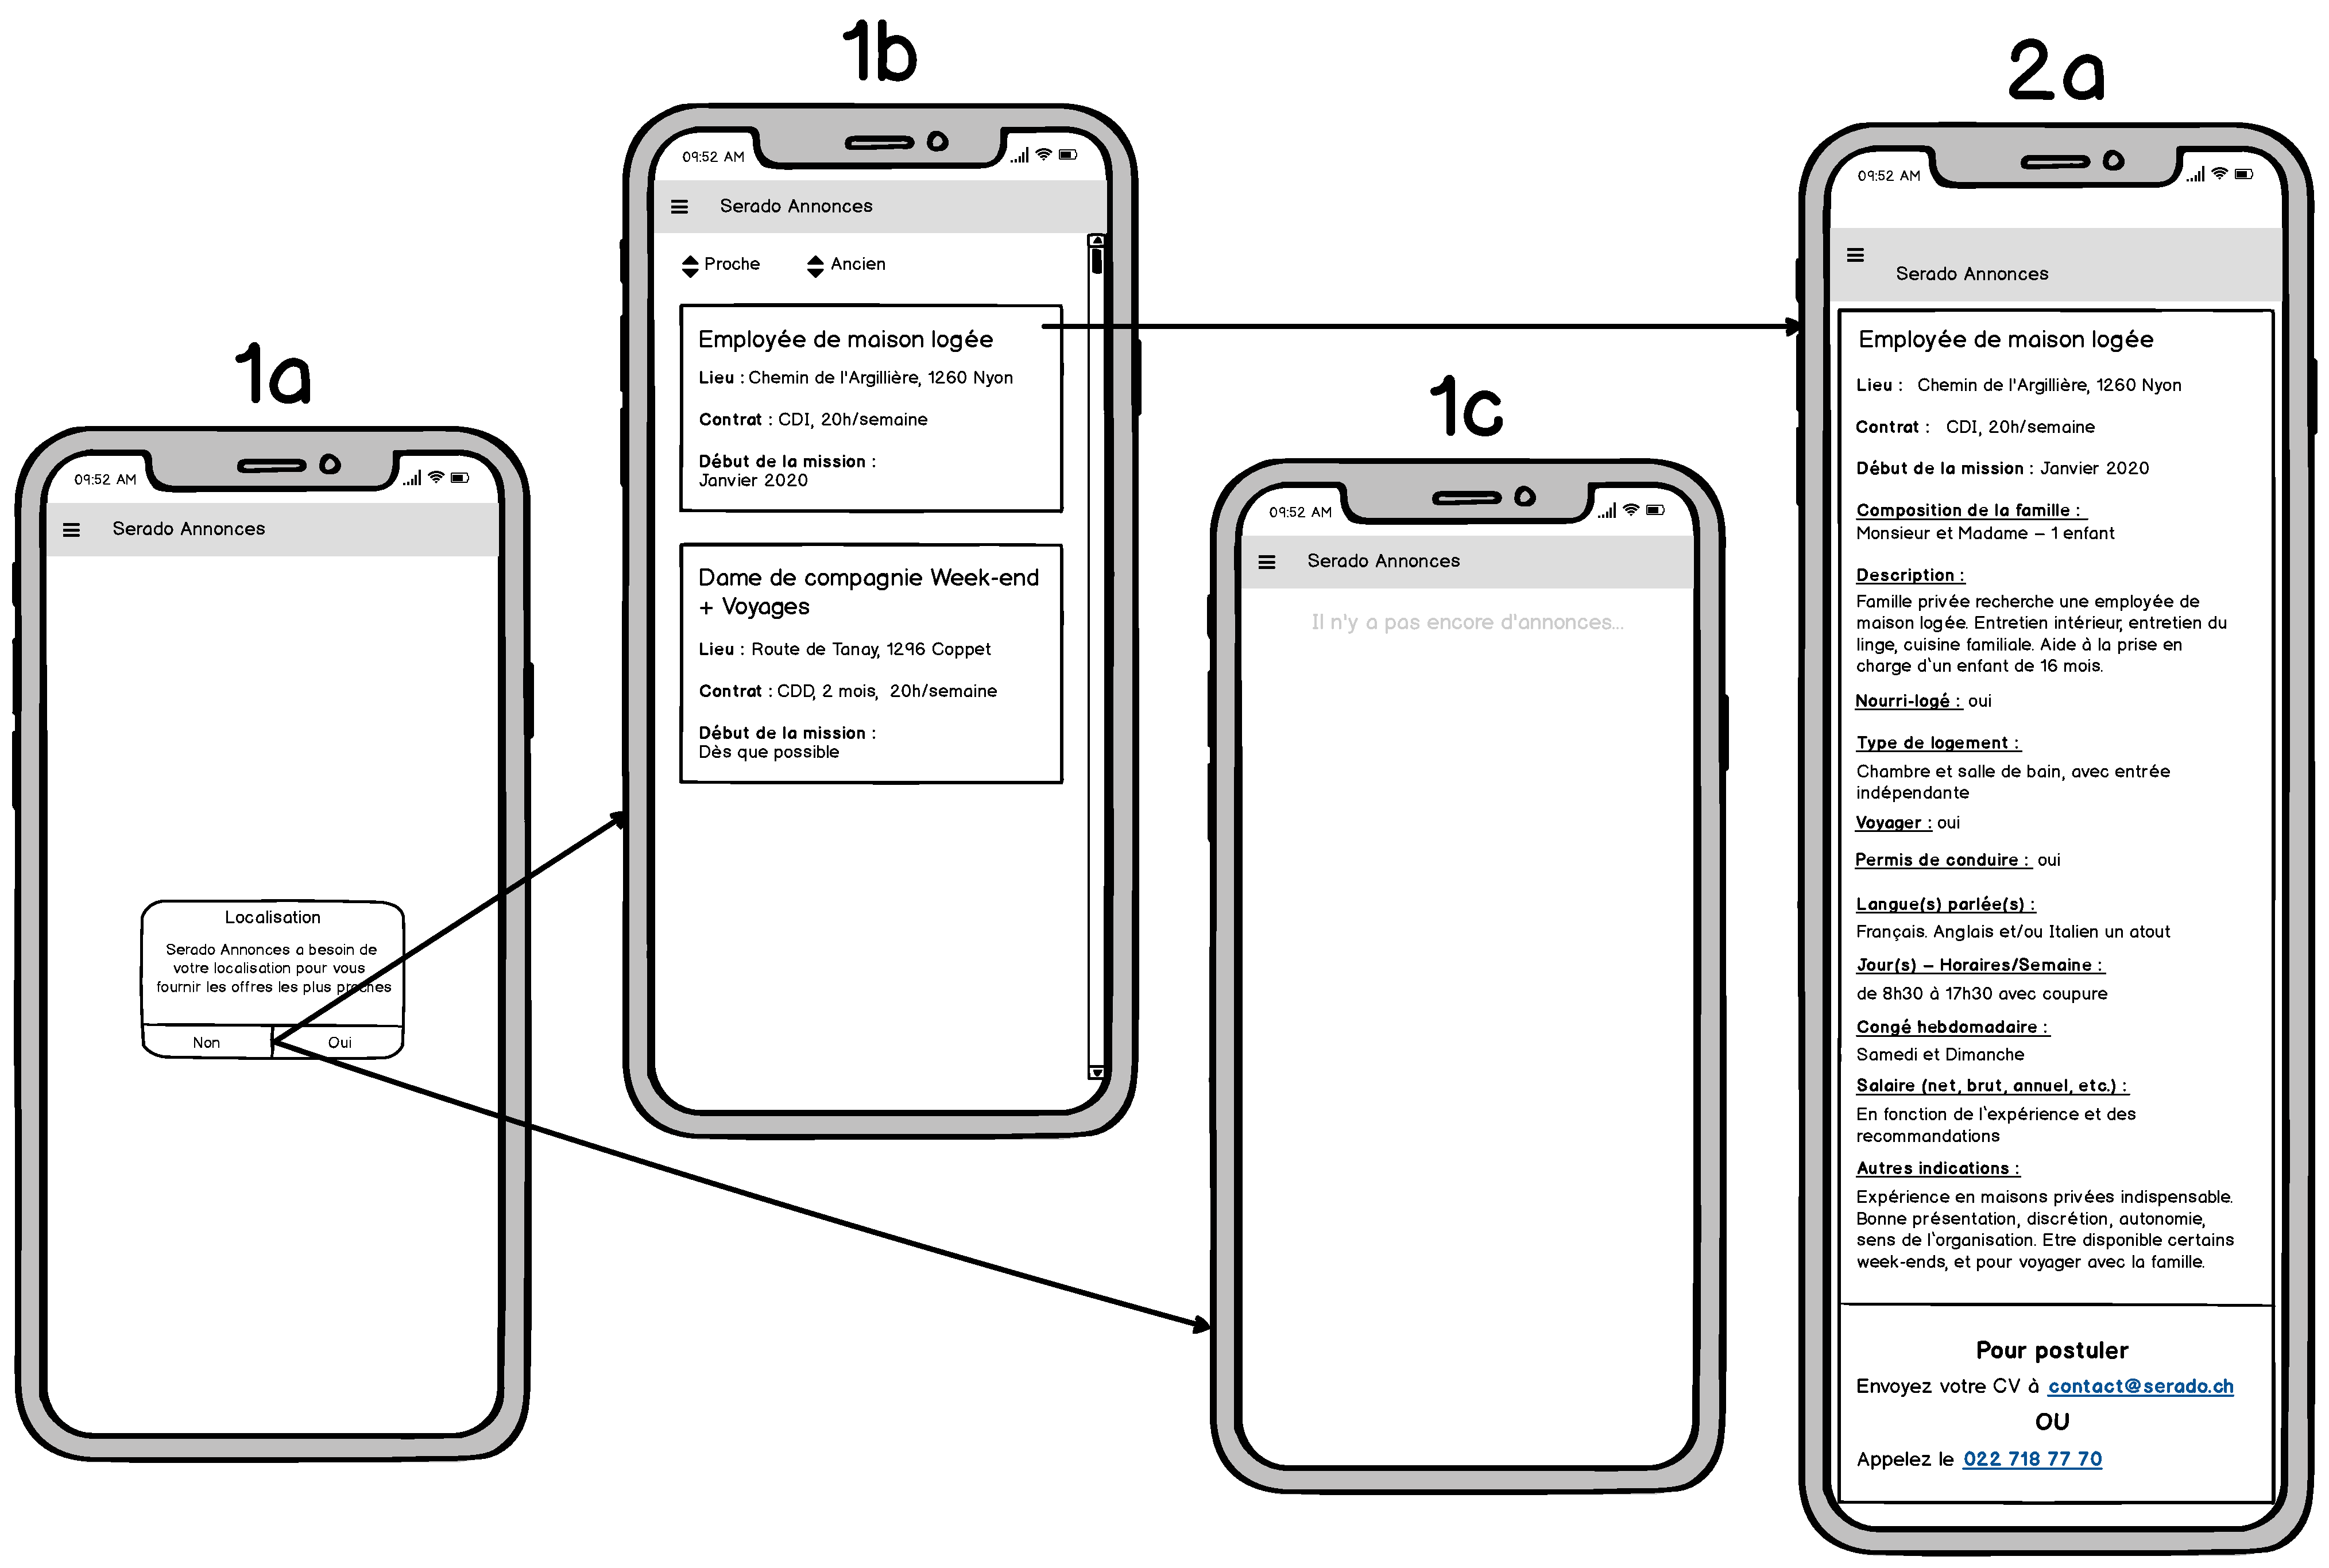
\includegraphics[width=\textwidth]{../mocks/1-2.pdf}
    \caption{Maquettes - Annonces}
    \label{fig:mockup_ads}
\end{figure}

\begin{figure}[H]
    \centering
    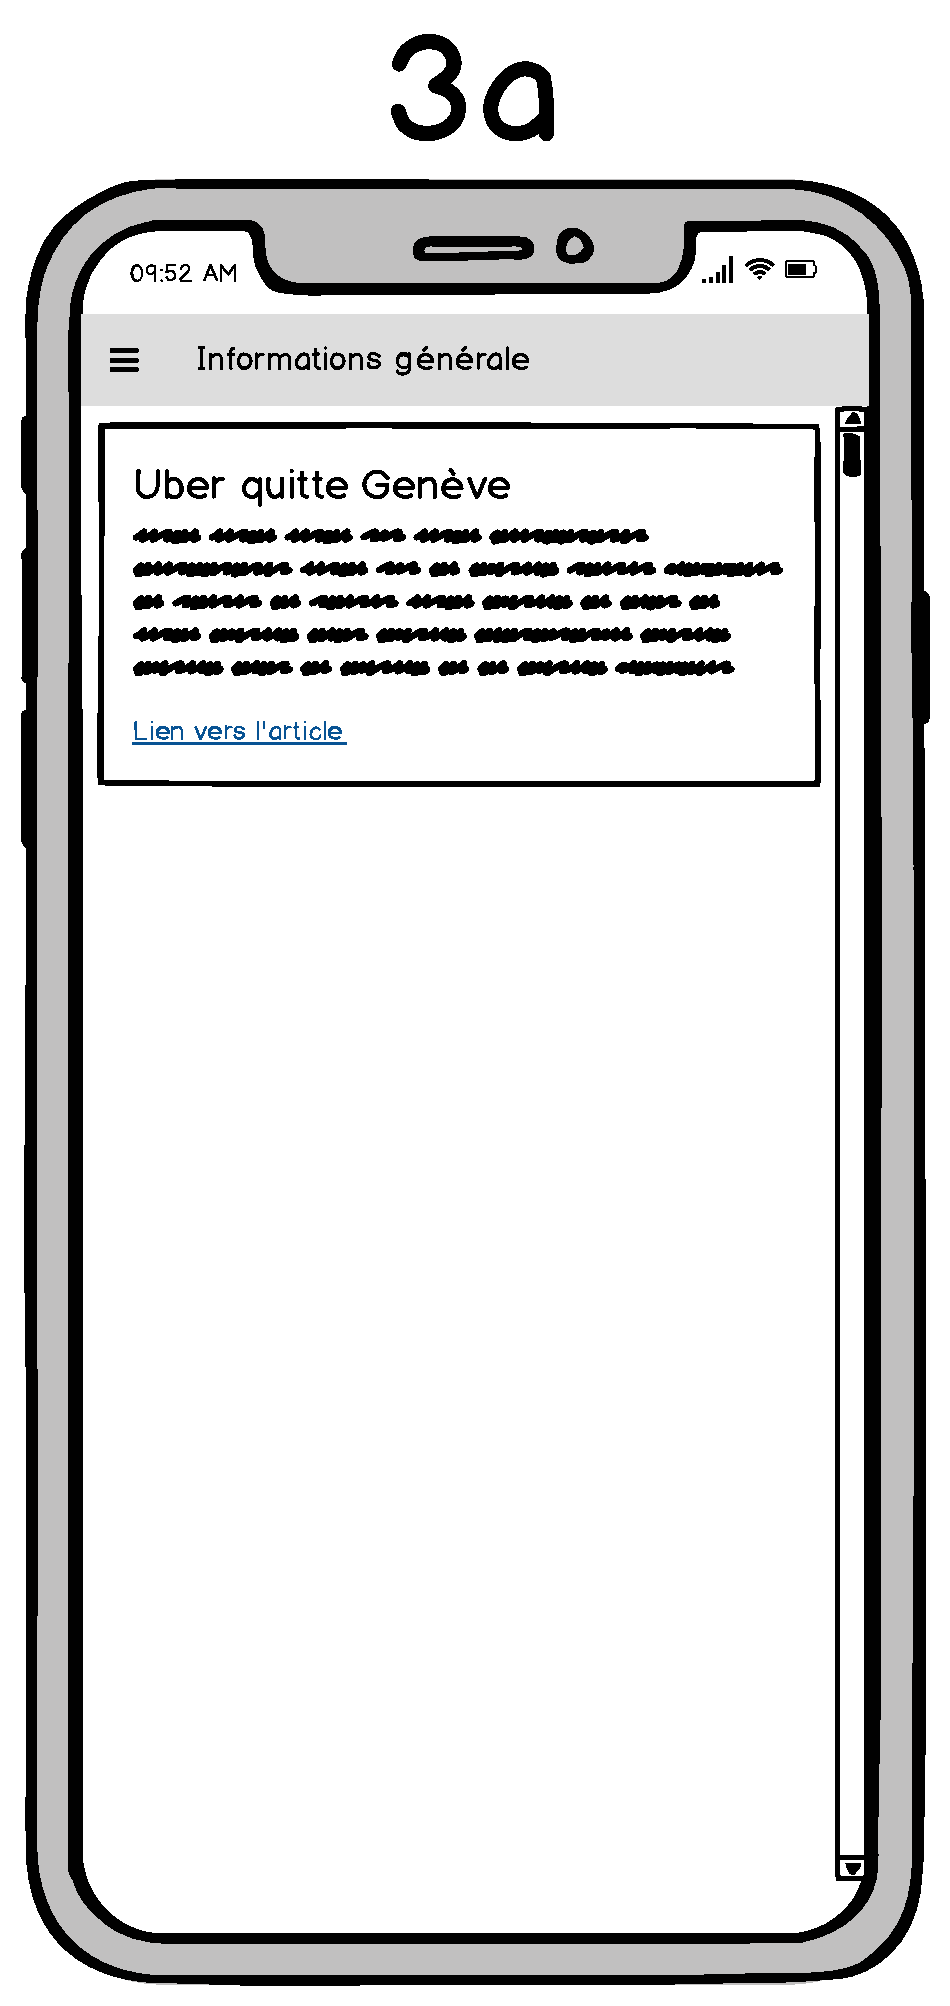
\includegraphics[width=0.25\textwidth]{../mocks/3.pdf}
    \caption{Maquettes - Informations générales}
    \label{fig:mockups_infos}
\end{figure}

\begin{figure}[H]
    \centering
    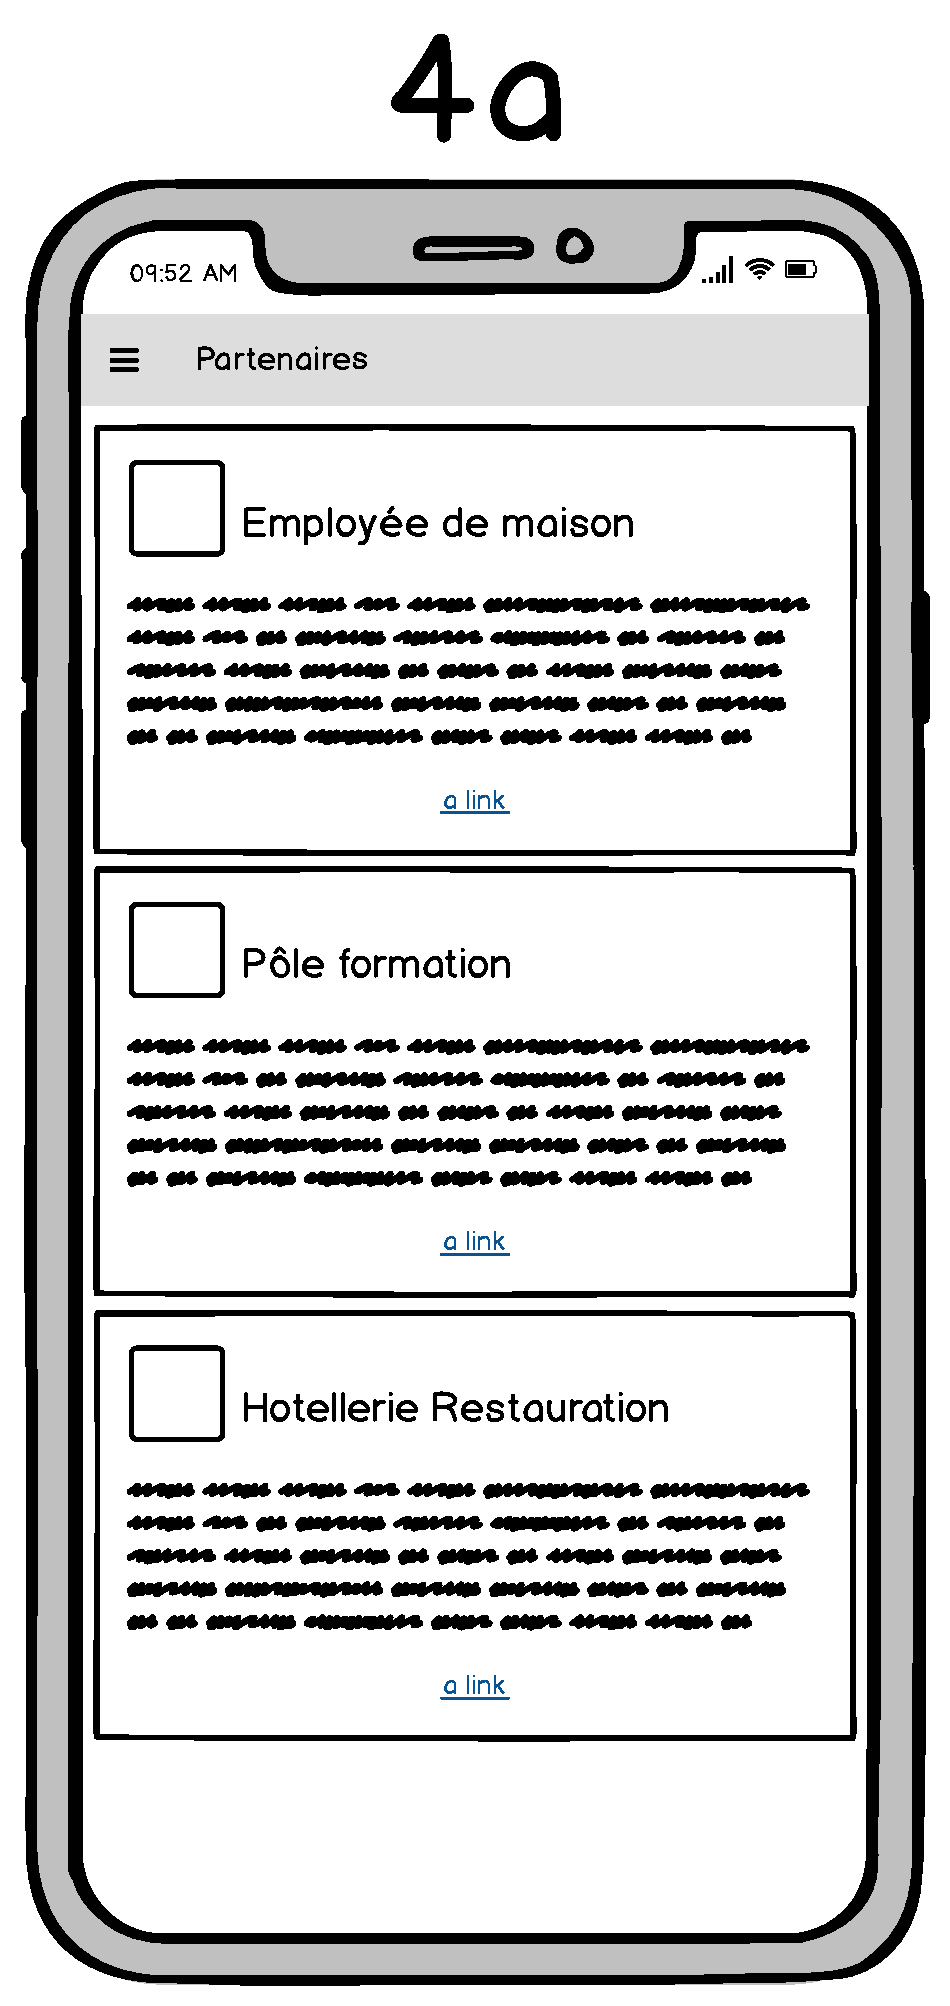
\includegraphics[width=0.25\textwidth]{../mocks/4.pdf}
    \caption{Maquettes - Partenaires}
    \label{fig:mockups_partners}
\end{figure}

\begin{figure}[H]
    \centering
    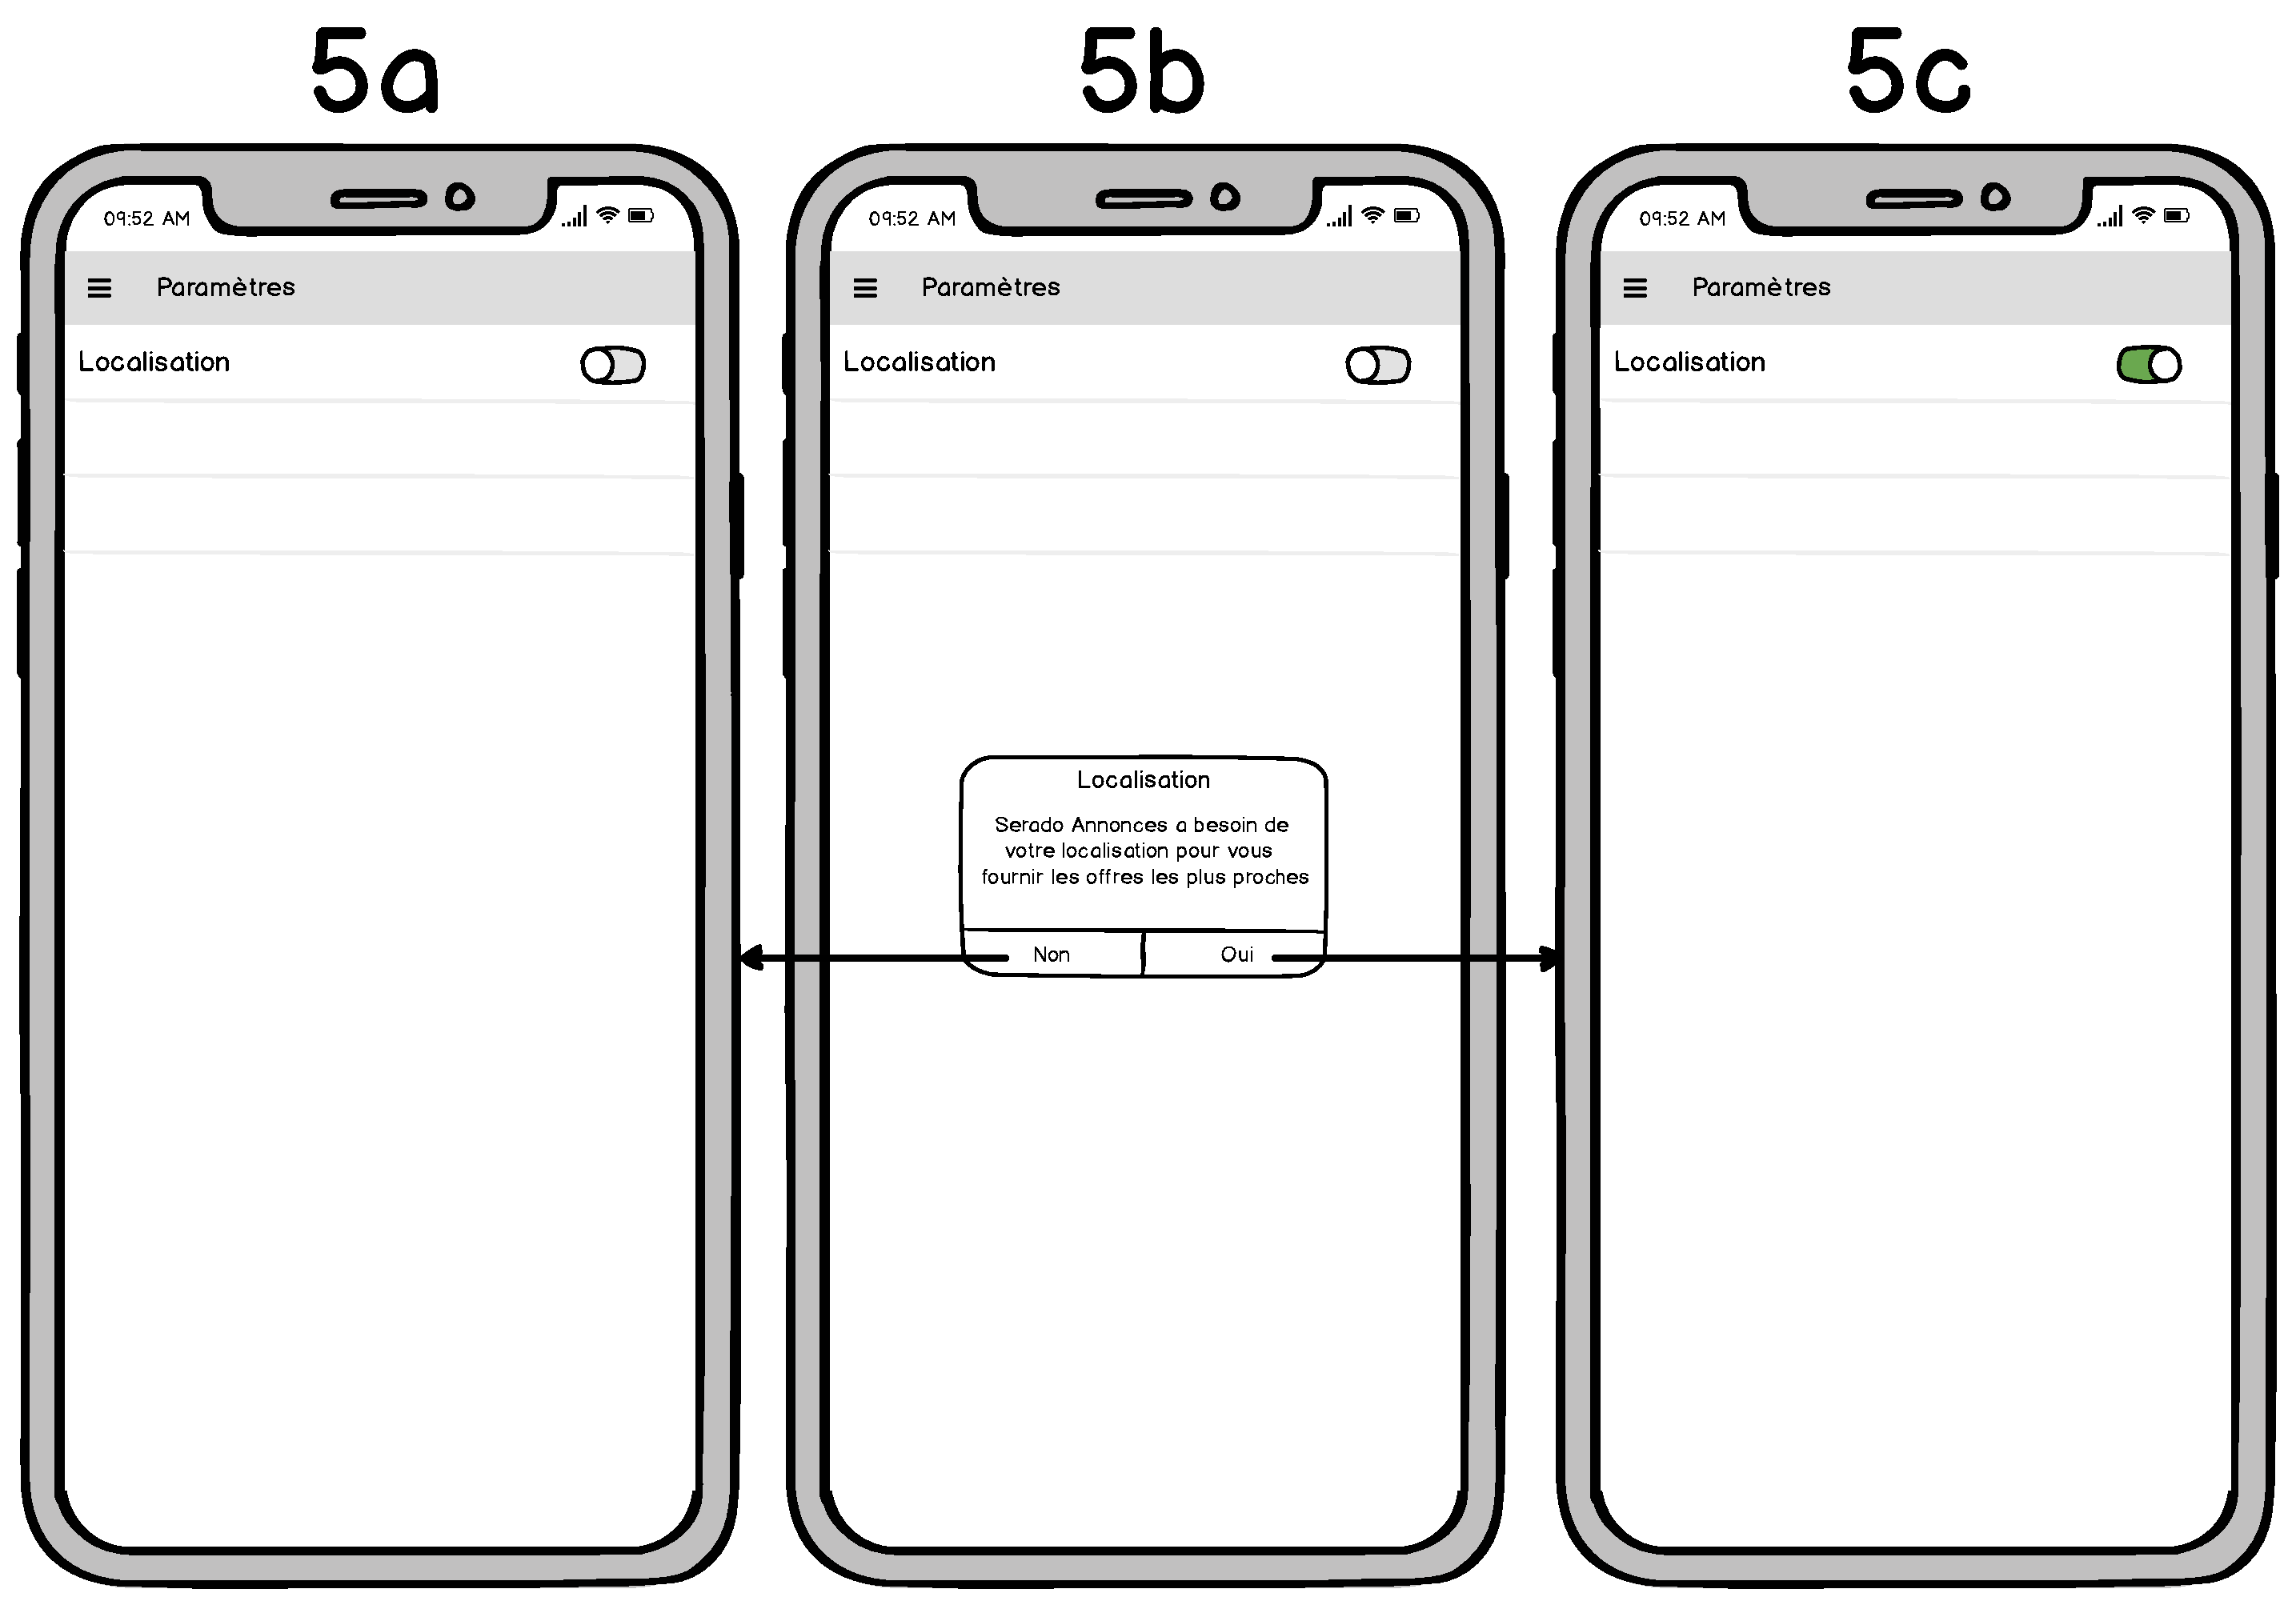
\includegraphics[width=0.8\textwidth]{../mocks/5.pdf}
    \caption{Maquettes - Paramètres}
    \label{fig:mockups_partners}
\end{figure}

Il est préférable d'ouvrir directement le fichier \verb|pdf| afin de mieux voir
chacun des écrans.

\section{Traitement des listes}
Vu que le nombre maximal d'objet dans une liste est d'environ 50 (50 annonces).
Nous pouvons récupérer directement tous les éléments de la liste à partir de la base
de données. Pas besoin de s'embêter avec un système de pagination.

Les listes (\textbf{annonces} \& \textbf{infos générales}) seront rafraîchie dans 
les cas de figure suivants:
\begin{itemize}
    \item \textit{Pull to refresh}\footnote{\textit{Swipe} vers le bas lorsque l'on
    se trouve en haut d'une liste}.
    \item Lorsque l'écran se charge pour la première fois.
    \item Lorsque une page s'affiche, alors que cela fait plus de 5 minutes qu'elle
    avait charger ses données.
    seulement si cela fait plus 
\end{itemize}

\section{Traitement de la position}
La position de l'utilisateur sera rafraîchie à chaque fois que la liste \textbf{annonces}
sera rafraîchie, si l'application a l'autorisation de localiser l'utilisateur.

\section{État global de l'application}
Nous utiliserons \textit{@ngrx/store} (\url{https://ngrx.io/guide/store}) afin de 
gérer l'état global de l'application.

Les éléments suivants devront être stockés:
\begin{itemize}
    \item \textbf{Liste des annonces}
    \item Heure du dernier chargement de la \textbf{liste des annonces}
    \item \textbf{Liste des informations générales}
    \item Heure du dernier chargement de la \textbf{liste des infos générales}
    \item La position GPS de l'utilisateur
\end{itemize}
\vspace{1em}

Le diagramme ci-dessous décrit le comportement principal de l'application, c'est-à-dire,
dans l'ordre:
\begin{enumerate}
    \item Charger (trouver) la position actuelle de l'utilisateur.
    \item Charger les annonces.
    \item Trouver et ajouter les coordonnées GPS de chacune des annonces (avec Google Maps API).
    \item Calculer et ajouter les distances entre la position actuelle de l'utilisateur et la position de chacune des annonces.
\end{enumerate}

\begin{figure}[H]
    \centering
    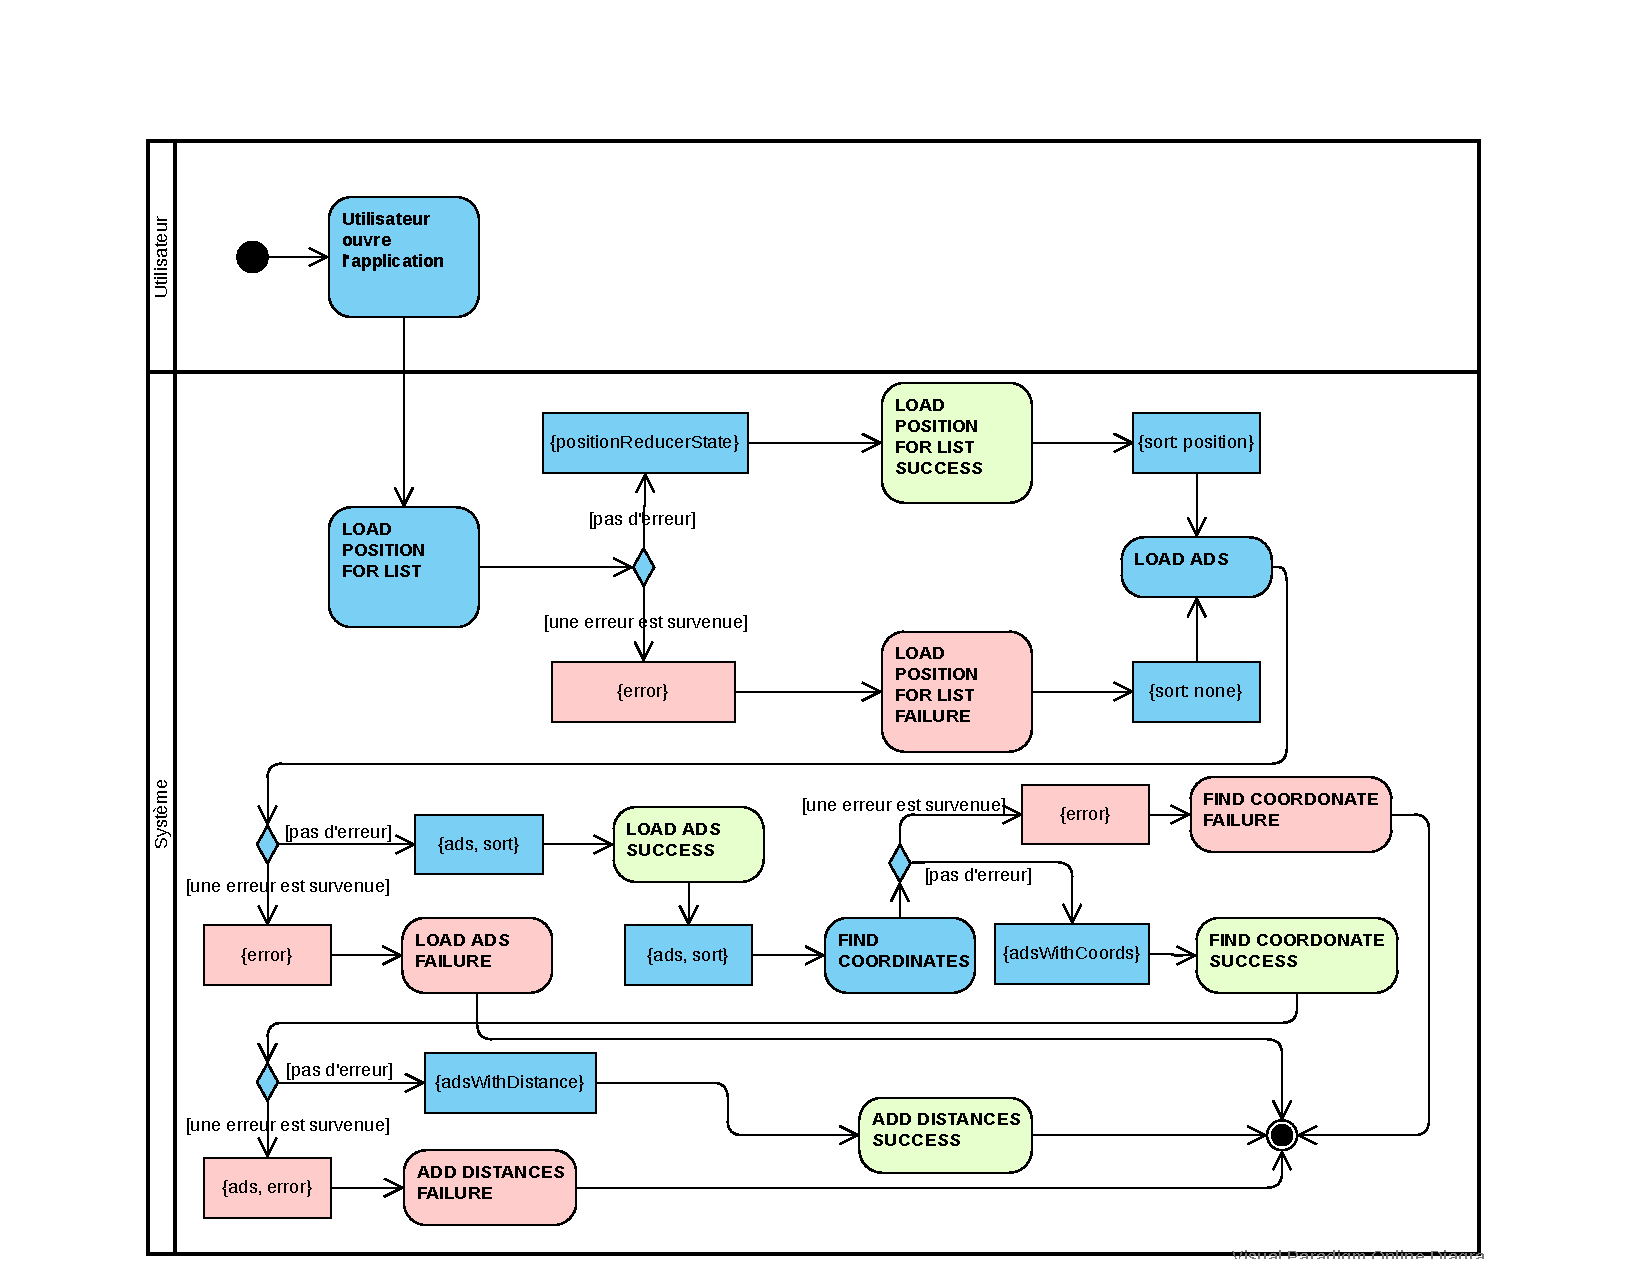
\includegraphics[width=\textwidth]{../diags/serado_activity.pdf}
    \caption{Diagramme d'activité}
    \label{fig:activity_diagram}
\end{figure}

Ces actions correspondes à des actions \textit{NgRx} et peuvent être trouvée dans le dossier
\verb|ngx-store/actions|.

\section{Paramètres de l'application}
Il n'y aura qu'un seul paramètre:
\begin{itemize}
    \item Activer/désactiver la localisation
\end{itemize}
Ceci permettra à l'utilisateur qui avec refuser l'accès à sa localisation de
l'autoriser plus tard s'il le souhaite.

\section{Requêtes HTTP}
Puisque l'application sera disponible à partir d'applications mobiles et du web,
il va falloir traiter les requêtes HTTP différemment:
\begin{itemize}
    \item Utiliser la classe \textit{HttpClient} pour les requêtes web
    \item Utiliser la classe \textit{HTTP} pour les requêtes mobiles
\end{itemize}
On créera une \textit{Factory} qui retournera le bon objet en fonction de la
plateforme où nous nous trouvons.

\begin{figure}[H]
    \centering
    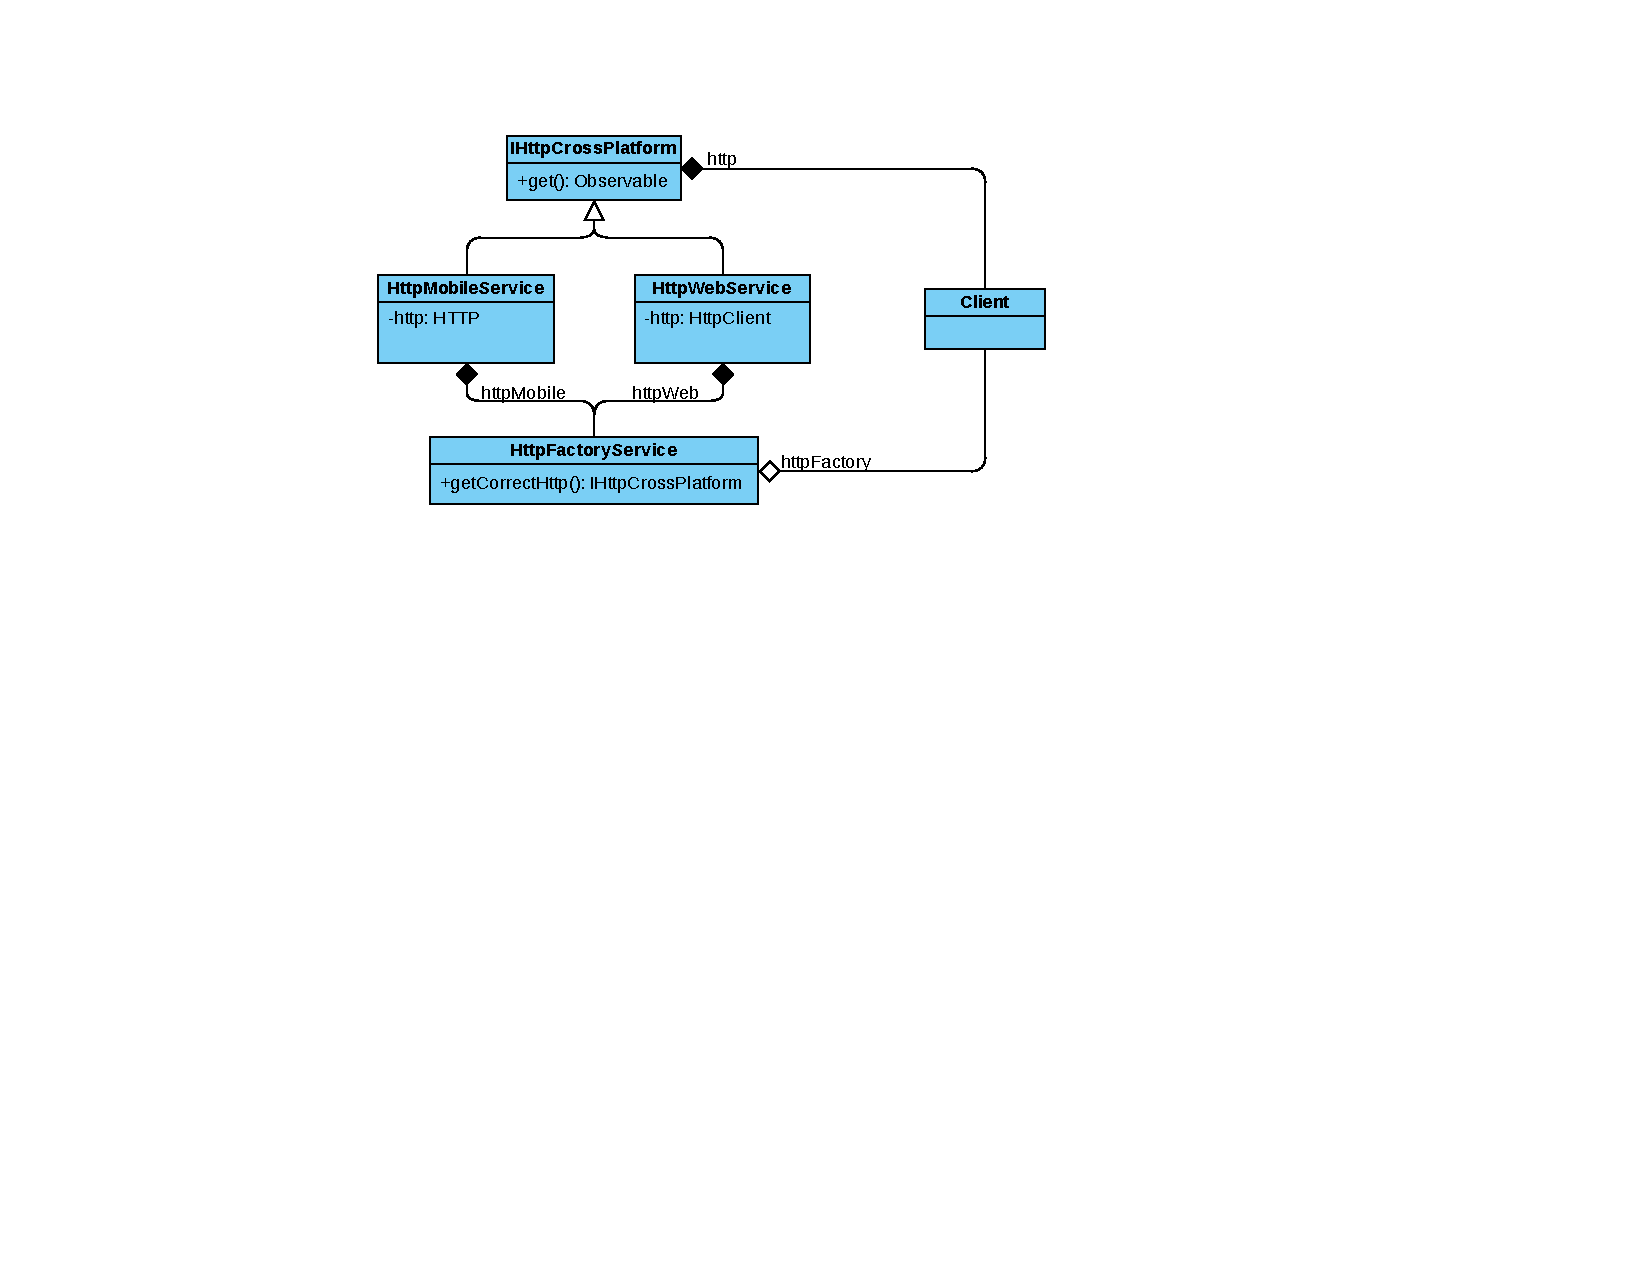
\includegraphics[width=0.7\textwidth]{../diags/http_factory_class.pdf}
    \caption{Diagramme de classe de la HttpFactory}
    \label{fig:class_http_factory}
\end{figure}

Un \textit{HttpInterceptor} sera aussi utilisé pour simuler les requêtes HTTP,
en attendant de maîtriser la génération (ou quelque chose à voir) d'API depuis
\textit{WordPress}.

\chapter{Déploiement}

Les déploiement consiste à faire passer les applications de l'état de développement
à l'état de production.

\section{Informations de connexion \& informations générales}
\begin{description}
    \item[Google Maps API] \verb|serado.dev@gmail.com : <mot de passe google>|
    \item[Android developer] \verb|serado.dev@gmail.com : <mot de passe google>|
    \item[Apple developer program] \verb|reception@serado.ch : <mot de passe du compte apple>| 
    \item[D-U-N-S (numéro d'identification de l'entreprise)] 481938681
\end{description}

Les mots de passes sont connus de l'entreprise.

\section{Sécurisation des Maps API Key}\label{sec:api_key}
Afin d'éviter une utilisation de la API Key non autorisée, il faut restreindre
l'utilisation de la clé aux appareils autorisés:
\begin{enumerate}
    \item Se rendre sur \url{https://console.cloud.google.com}\label{cloud}
    \item Sur la gauche, \verb|API et Services|
    \item Sur la gauche, \verb|Identifiants|
\end{enumerate}
Ici sont représentées les clés. Il y en une pour l'application Android ainsi qu'une
autre pour l'application iOS.

\section{Surveillances des coûts}
L'utilisation des services Google Maps est gratuite jusqu'à un certain montant.
Vous pouvez surveiller ce montant à partir de \url{https://console.cloud.google.com}.

\section{Stores}
Cette section détaille la mise sur les stores (Play Store \& App Store).

\subsection{Android} \label{sec:android}
Dans un premier temps, il s'agira de créer une APK signée.
\begin{verbatim}
    ionic cordova build android --prod --release
\end{verbatim}
Cette commande permet de gérer une APK non signée. Voir le contenu du dossier
\verb|serado_keystore| (\verb|readme.txt|) pour voir comment signer l'APK.

Ce dossier se trouve dans le compte Google Drive du compte
\url{serado.dev@gmail.com}

\begin{enumerate}
    \item Création d'un compte Android Developer (25\$)
    \item Remplissage de tous les champs nécessaires (à gauche)\label{all_fileds}
    \item Importer l'APK signée
\end{enumerate}

\textbf{Si l'application doit être mise à jour, il faut que la nouvelle version de
l'application soit signée avec le contenu du dossier} \verb|serado_keystore|

\subsection{iOS}
Pour générer l'application:
\begin{verbatim}
    ionic cordova prepare ios
\end{verbatim}

\begin{enumerate}
    \item Obtention du numéro D-U-N-S
    \item Création du compte Apple Developer Program
\end{enumerate}

\section{Aide}

\begin{itemize}
    \item Changer la description, l'image ou les captures d'écran de l'application
    $\rightarrow$ pt. \ref{all_fileds} de la section \ref{sec:android}
    \item Regarder les coûts actuels de l'API Google Maps $\rightarrow$ pt. \ref{cloud} de la section \ref{sec:api_key}
\end{itemize}

\end{document}

